\documentclass[12pt]{article}
\usepackage{graphicx}
\usepackage{latexsym}
\usepackage{amssymb}
\usepackage[utf8]{inputenc}
\usepackage[T1]{fontenc}
\usepackage[french]{babel}
\usepackage[french,algoruled,vlined]{algorithm2e}

\setlength{\textheight}{240mm}
\setlength{\textwidth}{162mm}
\setlength{\topmargin}{-11mm}
\setlength{\oddsidemargin}{+1mm}
\setlength{\unitlength}{1cm}

\begin{document}
\noindent
{\bf Département d'informatique \hfill Architecture} \\
$3^{\grave{e}me}$ année
\vspace*{1cm}
\begin{center}
{\large \bf Architecture \emph{MIPS} mono-cycle}
\end{center}

\renewcommand{\labelitemi}{$\bullet$}
\renewcommand{\labelitemii}{$\star$}

Nous allons réaliser une architecture simple où toutes les instructions s'exécuteront en un cycle. De plus, le code et les données
seront placés dans des mémoires séparées.

\section{Modèle de programmation}

\subsection{Espace d'adressage}

Le bus d'adresse de la machine \emph{MIPS} que nous étudions est de $32$ bits et l'unité élémentaire
de mémorisation est l'octet. On peut donc accéder à $2^{32}$ octets. En fait,
pour cette implémentation nous aurons deux mémoires séparées~: une pour les instructions et une pour les données. Nous aurons
donc accès à $2^{32}$ octets pour chacune des mémoires.

\subsection{Registres}

Nous présentons dans la table \ref{table:registers}
les $32$ registres que comporte l'unité centrale de cette architecture. La première colonne de cette table indique
le nom utilisé en assembleur pour décrire ce registre, la deuxième colonne donne le numéro du registre et
la dernière indique l'usage qui en est généralement fait.

\begin{table}[!htpb]
\begin{center}
\begin{tabular}{|c|c|p{11.5cm}|}
\hline
Nom & Numéro & Usage\\
\hline
\hline
\$zero & $0$ & la constante zéro\\
\hline
\$at & $1$ & réservé pour l'assembleur\\
\hline
\$v0 & $2$ & évaluation d'une expression et résultat d'une fonction\\
\hline
\$v1 & $3$ & évaluation d'une expression et résultat d'une fonction\\
\hline
\$a0 & $4$ & premier argument d'une fonction\\
\hline
\$a1 & $5$ & deuxième argument d'une fonction\\
\hline
\$a2 & $6$ & troisième argument d'une fonction\\
\hline
\$a3 & $7$ & quatrième argument d'une fonction\\
\hline
\$t0 & $8$ & temporaire (n'est pas préservé lors de l'appel d'une fonction)\\
\hline
\$t1 & $9$ & temporaire (n'est pas préservé lors de l'appel d'une fonction)\\
\hline
\$t2 & $10$ & temporaire (n'est pas préservé lors de l'appel d'une fonction)\\
\hline
\$t3 & $11$ & temporaire (n'est pas préservé lors de l'appel d'une fonction)\\
\hline
\$t4 & $12$ & temporaire (n'est pas préservé lors de l'appel d'une fonction)\\
\hline
\$t5 & $13$ & temporaire (n'est pas préservé lors de l'appel d'une fonction)\\
\hline
\$t6 & $14$ & temporaire (n'est pas préservé lors de l'appel d'une fonction)\\
\hline
\$t7 & $15$ & temporaire (n'est pas préservé lors de l'appel d'une fonction)\\
\hline
\$s0 & $16$ & temporaire et sauvegardé (est préservé lors de l'appel d'une fonction)\\
\hline
\$s1 & $17$ & temporaire et sauvegardé (est préservé lors de l'appel d'une fonction)\\
\hline
\$s2 & $18$ & temporaire et sauvegardé (est préservé lors de l'appel d'une fonction)\\
\hline
\$s3 & $19$ & temporaire et sauvegardé (est préservé lors de l'appel d'une fonction)\\
\hline
\$s4 & $20$ & temporaire et sauvegardé (est préservé lors de l'appel d'une fonction)\\
\hline
\$s5 & $21$ & temporaire et sauvegardé (est préservé lors de l'appel d'une fonction)\\
\hline
\$s6 & $22$ & temporaire et sauvegardé (est préservé lors de l'appel d'une fonction)\\
\hline
\$s7 & $23$ & temporaire et sauvegardé (est préservé lors de l'appel d'une fonction)\\
\hline
\$t8 & $24$ & temporaire (n'est pas préservé lors de l'appel d'une fonction)\\
\hline
\$t9 & $25$ & temporaire (n'est pas préservé lors de l'appel d'une fonction)\\
\hline
\$k0 & $26$ & réservé pour le système d'exploitation\\
\hline
\$k1 & $27$ & réservé pour le système d'exploitation\\
\hline
\$gp & $28$ & pointeur vers la zone des variables globales\\
\hline
\$sp & $29$ & pointeur de pile\\
\hline
\$fp & $30$ & pointeur vers la zone \emph{frame pointer}\\
\hline
\$ra & $31$ & adresse de retour d'une fonction\\
\hline
\end{tabular}
\end{center}
\caption{Les $32$ registres de la machine \emph{MIPS}}
\label{table:registers}
\end{table}

\subsection{Jeu d'instructions}

Nous allons étudier un sous-ensemble du jeux d'instructions de
l'architecture \emph{MIPS} $32$ bits, afin de pouvoir réaliser l'architecture de cet ordinateur.
Les instructions que nous allons étudier seront de trois types~:
\begin{itemize}
\item les instructions de référence à la mémoire \emph{load word} (\verb+lw+) et \emph{save word} (\verb+sw+)~;
\item les instructions arithmétiques et logiques \verb+add+, \verb+sub+, \verb+and+, \verb+or+ et \verb+slt+~;
\item les instructions de saut \emph{branch equal} (\verb+beq+) et \emph{jump} (\verb+j+).
\end{itemize}

Nous allons maintenant décrire les différentes instructions et donner leur format. Notons
que toutes les instructions sont codées sur $32$ bits.

\begin{itemize}

\item \verb+lw $s1, 100($s2)+\\
Soit $a$ la valeur du registre $s2$ plus $100$.
Cette instruction charge le mot de $32$ bits commençant à l'adresse $a$ dans le registre \verb+$s1+.
L'instruction \verb+lw rt, v(rs)+ est codée en langage machine~:\\
\begin{center}
\begin{tabular}{cccc}
\hline
\multicolumn{1}{|c}{100011} & \multicolumn{1}{|c}{rs} & \multicolumn{1}{|c}{rt} & \multicolumn{1}{|c|}{v}\\
\hline
$6$ bits & $5$ bits & $5$ bits & $16$ bits\\
&&&\\
\end{tabular}
\end{center}

Notons que \verb+v+ est sur $16$ bits et peut donc représenter des déplacements de $-2^{15}=-32768$ à $2^{15}-1=32767$\\

\item \verb+sw $s1, 100($s2)+\\
Soit $a$ la valeur du registre $s2$ plus $100$.
Cette instruction sauvegarde le mot de $32$ bits contenu dans le registre \verb+$s1+ à l'adresse $a$.
L'instruction \verb+sw rt, v(rs)+ est codée en langage machine~:\\
\begin{center}
\begin{tabular}{cccc}
\hline
\multicolumn{1}{|c}{101011} & \multicolumn{1}{|c}{rs} & \multicolumn{1}{|c}{rt} & \multicolumn{1}{|c|}{v}\\
\hline
$6$ bits & $5$ bits & $5$ bits & $16$ bits\\
&&&\\
\end{tabular}
\end{center}

\item \verb+add $s1, $s2, $s3+\\
Cette instruction place dans le registre \verb+$s1+ la somme du registre \verb+$s2+ et \verb+$s3+.
L'instruction \verb+add rd, rs, rt+ est codée en langage machine~:\\
\begin{center}
\begin{tabular}{cccccc}
\hline
\multicolumn{1}{|c}{000000} & \multicolumn{1}{|c}{rs} & \multicolumn{1}{|c}{rt} & \multicolumn{1}{|c|}{rd} & \multicolumn{1}{|c|}{0} & \multicolumn{1}{|c|}{100000}\\
\hline
$6$ bits & $5$ bits & $5$ bits & $5$ bits & $5$ bits & $6$ bits\\
&&&&&\\
\end{tabular}
\end{center}

Notons les $6$ premiers bits (qui représentent l'\emph{opcode}) des instructions arithmétiques et logiques sont toujours à $0$. Ce qui différencie ces
différentes instructions est la valeur des $6$ derniers bits de l'instruction (qui se nomme \emph{funct}).\\

\item \verb+sub $s1, $s2, $s3+\\
Cette instruction place dans le registre \verb+$s1+ la différence entre le registre \verb+$s2+ et le registre \verb+$s3+ (\verb+$s2+ - \verb+$s3+).
L'instruction \verb+sub rd, rs, rt+ est codée en langage machine~:\\
\begin{center}
\begin{tabular}{cccccc}
\hline
\multicolumn{1}{|c}{000000} & \multicolumn{1}{|c}{rs} & \multicolumn{1}{|c}{rt} & \multicolumn{1}{|c|}{rd} & \multicolumn{1}{|c|}{0} & \multicolumn{1}{|c|}{100010}\\
\hline
$6$ bits & $5$ bits & $5$ bits & $5$ bits & $5$ bits & $6$ bits\\
&&&&&\\
\end{tabular}
\end{center}

Notons les $6$ premiers bits (qui représentent l'\emph{opcode}) des instructions arithmétiques et logiques sont toujours à $0$. Ce qui différencie ces
différentes instructions est la valeur des $6$ derniers bits de l'instruction (qui se nomme \emph{funct}).\\

\item \verb+and $s1, $s2, $s3+\\
Cette instruction place dans le registre \verb+$s1+ le \emph{et logique bit à bit}
des registres \verb+$s2+ et \verb+$s3+ (\verb+$s2+ $\wedge$ \verb+$s3+).
L'instruction \verb+and rd, rs, rt+ est codée en langage machine~:\\
\begin{center}
\begin{tabular}{cccccc}
\hline
\multicolumn{1}{|c}{000000} & \multicolumn{1}{|c}{rs} & \multicolumn{1}{|c}{rt} & \multicolumn{1}{|c|}{rd} & \multicolumn{1}{|c|}{0} & \multicolumn{1}{|c|}{100100}\\
\hline
$6$ bits & $5$ bits & $5$ bits & $5$ bits & $5$ bits & $6$ bits\\
&&&&&\\
\end{tabular}
\end{center}

\item \verb+or $s1, $s2, $s3+\\
Cette instruction place dans le registre \verb+$s1+ le \emph{ou logique bit à bit}
des registres \verb+$s2+ et \verb+$s3+ (\verb+$s2+ $\vee$ \verb+$s3+).
L'instruction \verb+or rd, rs, rt+ est codée en langage machine~:\\
\begin{center}
\begin{tabular}{cccccc}
\hline
\multicolumn{1}{|c}{000000} & \multicolumn{1}{|c}{rs} & \multicolumn{1}{|c}{rt} & \multicolumn{1}{|c|}{rd} & \multicolumn{1}{|c|}{0} & \multicolumn{1}{|c|}{100101}\\
\hline
$6$ bits & $5$ bits & $5$ bits & $5$ bits & $5$ bits & $6$ bits\\
&&&&&\\
\end{tabular}
\end{center}

\item \verb+slt $s1, $s2, $s3+\\
Si $($\verb+$s2+ $<$ \verb+$s3+$)$  alors \verb+$s1+ $= 1$ sinon \verb+$s1+ $= 0$
L'instruction \verb+slt rd, rs, rt+ est codée en langage machine~:\\
\begin{center}
\begin{tabular}{cccccc}
\hline
\multicolumn{1}{|c}{000000} & \multicolumn{1}{|c}{rs} & \multicolumn{1}{|c}{rt} & \multicolumn{1}{|c|}{rd} & \multicolumn{1}{|c|}{0} & \multicolumn{1}{|c|}{101010}\\
\hline
$6$ bits & $5$ bits & $5$ bits & $5$ bits & $5$ bits & $6$ bits\\
&&&&&\\
\end{tabular}
\end{center}

\item \verb+beq $0, $1, v+\\
Cette instruction permet de faire un saut conditionel relativement à la valeur du compteur ordinal (\verb+PC+).
Si \verb+$s0+ $=$ \verb+$s1+ la prochaine instruction sera cherchée en \verb+PC+ $+\ 4 + v \times 4$ sinon elle sera cherchée en \verb+PC+ $+\ 4$.\\
Par exemple, soit le programme suivant~:\\
\begin{verbatim}
8:  add $1,$2,$3
12: beq $0,$1,2
16: ...
20: ...
24: ...
28: ...
\end{verbatim}

Notons que les adresses des instructions vont de $4$ en $4$ car une instruction est sur $32$ bits. \`A la fin de l'exécution de l'instruction
\verb+beq $0,$1,2+, si \verb+$s0+ $=$ \verb+$s1+ on aura \verb+PC+ $= 12 + 4 + 4 * 2 = 24$ sinon on aura \verb+PC+ $= 16$.\\
L'instruction \verb+beq rs, rt, v+ est codée en langage machine~:\\
\begin{center}
\begin{tabular}{cccc}
\hline
\multicolumn{1}{|c}{000100} & \multicolumn{1}{|c}{rs} & \multicolumn{1}{|c}{rt} & \multicolumn{1}{|c|}{v}\\
\hline
$6$ bits & $5$ bits & $5$ bits & $16$ bits\\
&&&\\
\end{tabular}
\end{center}


\item \verb+j v+\\
Cette instruction permet de faire un saut inconditionel à l'adresse \verb+v+ (nous allons voir que c'est un peu plus compliqué).
L'instruction \verb+j v+ est codée en langage machine~:\\
\begin{center}
\begin{tabular}{cc}
\hline
\multicolumn{1}{|c}{000010} & \multicolumn{1}{|c|}{v}\\
\hline
$6$ bits & $26$ bits\\
&\\
\end{tabular}
\end{center}

On voit que la valeur de saut \verb+v+ est codée sur $26$ bits. Or, une adresse est sur $32$ bits. La valeur \verb+v+ est en fait multipliée par $4$ et
les $4$ bits de poids forts manquant sont les $4$ bits de poids forts de \verb+PC+ $+\ 4$.\\
Soit le programme suivant~:
\begin{verbatim}
Loop: 80000: ...
      80004: ...
      80008: ...
      80012: ...
      80016: ...
      80020: j Loop
      80024: ...
\end{verbatim}

L'instruction \verb+j Loop+ (qui permet de revenir à l'adresse \verb+80000+) est écrite de manière abusive, car dans l'instruction \verb+j Loop+, \verb+Loop+
ne vaut pas \verb+80000+. Néanmoins, on écrit de cette manière pour que ce soit plus lisible.
En fait, il faudrait écrire \verb+j 20000+ pour faire le saut correctement. En effet, la valeur de \verb+PC+ est de $80020$ donc celle de \verb+PC+ $+\ 4$
est de $80024$. Les $4$ bits de poids forts de $80024$ (sur $32$ bits) sont à zéro et donc le saut est effectué à l'adresse $20000 * 4$ sur $28$ bits
auxquels ont ajoute les $4$ bits de poids forts à zéro. On obtient donc bien l'adresse $80000$ sur $32$ bits.\\

\end{itemize}

\subsection{Exemple de programme}

Nous allons présenter un petit programme en langage C, puis sa traduction en assembleur et en langage machine.
\begin{verbatim}
if (i != j) f = g + h;
else f = g - h;
\end{verbatim}

Nous supposons que les variables \verb+f+, \verb+g+, \verb+h+, \verb+i+ et \verb+j+ sont représentées respectivement par les registres
\verb+$s0+, \verb+$s1+, \verb+$s2+, \verb+$s3+ et \verb+$s4+. De plus, nous supposons que le programme commence à l'adresse \verb+0+.
La traduction en assembleur de ce programme est la suivante~:

\begin{verbatim}
       0: beq $s3, $s4, Else
       4: add $s0, $s1, $s2
       8: j Exit
Else: 12: sub $s0, $s1, $s2
Exit: 16:
\end{verbatim}

Enfin, la traduction en langage machine donne le programme suivant~:

\begin{verbatim}
 0: 000100 10011 10100 0000000000000010
 4: 000000 10001 10010 10000 00000 100000
 8: 000010 00000000000000000000000100
12: 000000 10001 10010 10000 00000 100010
16:
\end{verbatim}

\subsection{Exercice}

Traduire en assembleur puis en langage machine le programme suivant~:

\begin{verbatim}
A[300] = h + A[300]
\end{verbatim}

On supposera que l'adresse de \verb+A+ est dans le registre \verb+$t1+ et la valeur de \verb+h+ dans le registre \verb+$s2+.

\section{Architecture}

L'architecture que nous allons présenter dans ce chapitre décodera et exécutera chaque instruction sur un seul cycle d'horloge. Pour ce
faire, nous aurons besoin de deux mémoires~: une pour les instructions et une pour les données.\\
Nous allons tout d'abord présenter les différents éléments de l'unité de traitement et les liens entre eux, puis l'unité de contrôle et
enfin nous parlerons des performances de cette architecture.

\subsection{Unité de traitement}

La figure \ref{fig:traitement1} présente les blocs principaux de l'unité de traitement. Nous allons détailler chacun de ces éléments.

\begin{figure}[!htpb]
\begin{center}
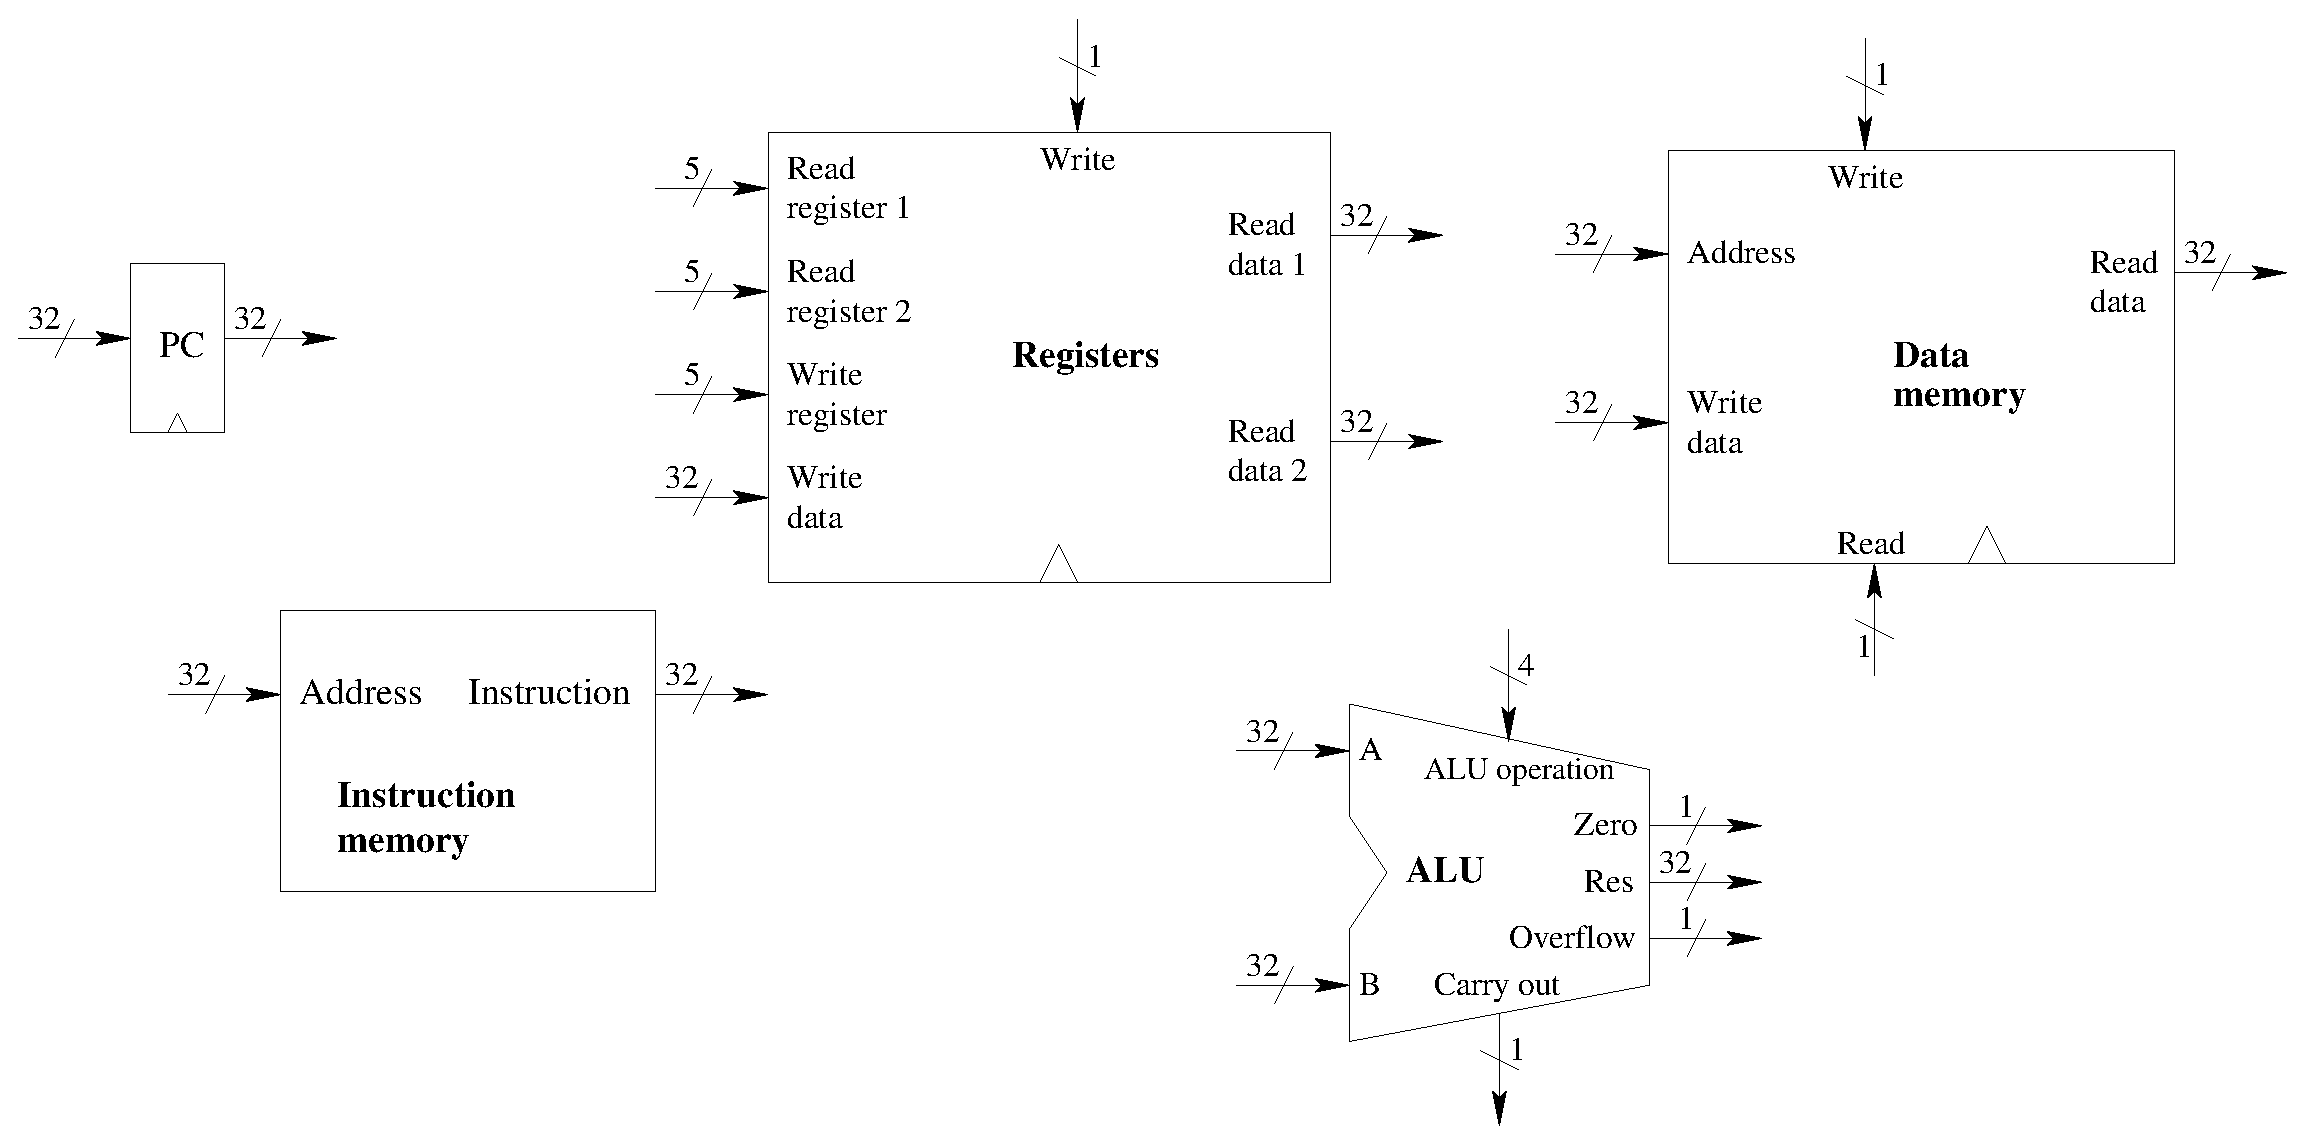
\includegraphics[width=16cm]{traitement1.eps}
\caption{Blocs principaux de l'unité de traitement}
\label{fig:traitement1}
\end{center}
\end{figure}


\subsubsection{Compteur ordinal (\texttt{PC})}

Le compteur ordinal est un registre de $32$ bits qui permet de stocker l'adresse
de la prochaine instruction à décoder et exécuter. L'entrée de ce registre est stockée à chaque
front montant de l'horloge.

\subsubsection{Mémoire des instructions (\emph{Instruction memory})}

La mémoire des instructions contiendra le programme. Elle met en sortie les $32$ bits commençant
à l'adresse spécifiée sur la broche \verb+Address+. Le contenu élémentaire de stockage de cette mémoire est l'octet,
mais on peut y lire des données de $8$, $16$ ou $32$ bits. On y lira ici toujours des valeurs sur $32$ bits.

\subsubsection{Mémoire des données (\emph{Data memory})}

La mémoire des données contiendra les données du programme. La mémoire met sur sa sortie \verb+Read data+ les $32$ bits de la mémoire
commençant à l'adresse \verb+Address+ si la broche \verb+Read+ est à \verb+1+. Si la broche \verb+Write+ est à \verb+1+, au front montant
de l'horloge, la donnée en entrée sur la broche \verb+Write data+ est copiée dans la mémoire à partir de l'adresse \verb+Address+. Le
comportement est indéfini si \verb+Read+ et \verb+Write+ sont tous les deux à \verb+1+.

\subsubsection{Banc de registres (\emph{Registers})}

Le banc de registre va contenir les $32$ registres de la machine \emph{MIPS}. La sortie \verb+Read data 1+ a pour valeur le contenu du registre
dont le numéro est donné sur la broche \verb+Read register 1+. La sortie \verb+Read data 2+ a pour valeur le contenu du registre
dont le numéro est donné sur la broche \verb+Read register 2+. La valeur présente sur l'entrée \verb+Write data+ sera copiée dans le
registre de numéro \verb+Write register+ au top d'horloge si l'entrée \verb+Write+ est à \verb+1+.\\

\textbf{Exercice 1~:} réaliser le banc de registres.

\subsubsection{Unité arithmétique et logique (\texttt{ALU})}

\begin{table}[!htpb]
\begin{center}
\begin{tabular}{|c|c|}
\hline
\verb+ALU operation+ & Fonction\\
\hline
\hline
\verb+0000+ & $A\wedge B$\\
\hline
\verb+0001+ & $A\vee B$\\
\hline
\verb+0010+ & $A+B$\\
\hline
\verb+0110+ & $A-B$\\
\hline
\verb+0111+ & si $A < B$ alors $1$ sinon $0$\\
\hline
\verb+1100+ & $\neg(A \vee B)$\\
\hline
\end{tabular}
\end{center}
\caption{Fonctionnement de l'unité arithmétique et logique}
\label{table:alu}
\end{table}

La table \ref{table:alu} décrit la valeur calculée sur la sortie \verb+Res+ en fonction des entrées \verb+A+, \verb+B+ et \verb+ALU operation+.
La sortie \verb+Zero+ est à \verb+1+ ssi \verb+Res+ est à \verb+0+, la sortie \verb+Carry out+ est à \verb+1+ ssi il y a une retenue
(notons que
cette broche n'aura de signification que si l'on effectue une addition, une soustraction).
La sortie \verb+Overflow+ est à \verb+1+ ssi il y a un débordement dans le calcul effectué par l'unité arithmétique et logique (notons que
cette broche n'aura de signification que s'il on effectue une addition, une soustraction ou une comparaison). La table \ref{table:overflow} indique comment
se calcule un débordement en complément à deux.

\begin{table}[!htpb]
\begin{center}
\begin{tabular}{|c|c|c|c|}
\hline
Opération & A & B & Il y a débordement ssi le résultat est:\\
\hline
\hline
$A+B$ & $\ge 0$ & $\ge 0$ & $< 0$\\
\hline
$A+B$ & $< 0$ & $< 0$ & $\ge 0$\\
\hline
$A-B$ & $\ge 0$ & $< 0$ & $< 0$\\
\hline
$A-B$ & $< 0$ & $\ge 0$ & $\ge 0$\\
\hline
\end{tabular}
\end{center}
\caption{Détection d'un débordement}
\label{table:overflow}
\end{table}

\textbf{Exercice 2~:} réaliser l'unité arithmétique et logique.

\subsubsection{Connexions entre les différents éléments de l'unité de traitement}

\textbf{Exercice 3~:} ajouter les connexions et les composants nécessaires pour mettre à jour le compteur
ordinal \verb+PC+.\\

\textbf{Exercice 4~:} ajouter les connexions et les composants nécessaires pour relier la mémoire des instructions
au banc de registres.\\

\textbf{Exercice 5~:} ajouter les connexions et les composants nécessaires pour relier la mémoire des instructions
et le banc de registres à l'unité arithmétique et logique.\\

\textbf{Exercice 6~:} relier l'unité arithmétique et logique à la mémoire des données.\\

\textbf{Exercice 7~:} relier l'unité arithmétique et logique et la mémoire des données au banc de registres.\\

\subsection{Unité de contrôle}

\subsubsection{Contrôle de l'unité arithmétique et logique}

Pour simplifier la réalisation de l'unité de contrôle, nous allons tout d'abord réaliser une sous-unité de contrôle qui gèrera l'entrée \verb+ALU operation+
de l'unité de traitement. Comme indiqué dans la figure \ref{fig:alu-control}, cette sous-unité, que l'on nommera \emph{ALU control}, prend en entrée
les bits $5$ à $0$ de l'instruction (ces bits correspondent au champ \verb+funct+ d'une instruction arithmétique ou logique) et une sortie de l'unité
de contrôle \verb+ALUOp+ permettant d'indiquer le type de l'instruction (instruction de sauvegarde/chargement, instruction de saut conditionel, ou
instruction arithmétique ou logique). La table \ref{table:aluop} présente la relation entre la partie \verb+funct+ de l'instruction,
la sortie \verb+ALUOp+ de l'unité de contrôle et l'entrée \verb+ALU operation+
de l'unité arithmétique et logique.

\begin{figure}[!htpb]
\begin{center}
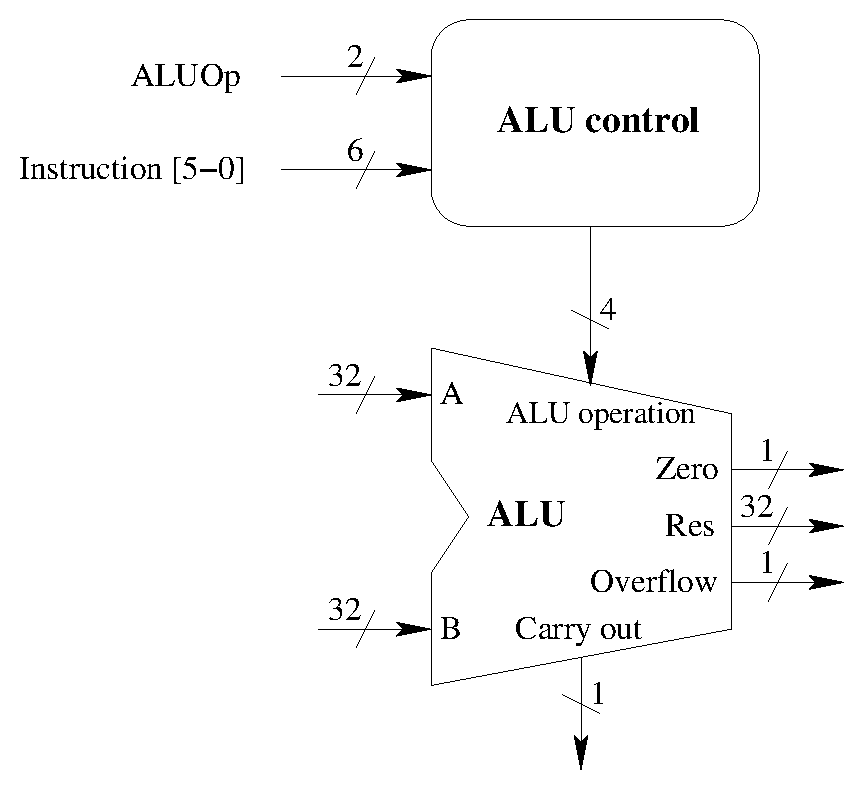
\includegraphics[width=8cm]{alu-control.eps}
\caption{Sous-unité de contrôle permettant de gérer l'unité arithmétique et logique}
\label{fig:alu-control}
\end{center}
\end{figure}

\begin{table}[!htpb]
\begin{center}
\begin{tabular}{|c|c|c|c|c|c|}
\hline
Opcode & ALUOp & Instruction & Champs \verb+funct+ & action de l'\verb+ALU+ & \verb+ALU operation+ \\
\hline
\hline
\verb+0x23+ & \verb+00+ & \verb+lw+ & \verb+XXXXXX+ & $+$ & \verb+0010+\\
\hline
\verb+0x2B+ & \verb+00+ & \verb+sw+ & \verb+XXXXXX+ & $+$ & \verb+0010+\\
\hline
\verb+0x04+ & \verb+01+ & \verb+beq+ & \verb+XXXXXX+ & $-$ & \verb+0110+\\
\hline
\verb+0+ & \verb+10+ & \verb+add+ & \verb+100000+ & $+$ & \verb+0010+\\
\hline
\verb+0+ & \verb+10+ & \verb+sub+ & \verb+100010+ & $-$ & \verb+0110+\\
\hline
\verb+0+ & \verb+10+ & \verb+and+ & \verb+100100+ & $\wedge$ & \verb+0000+\\
\hline
\verb+0+ & \verb+10+ & \verb+or+ & \verb+100101+ & $\vee$ & \verb+0001+\\
\hline
\verb+0+ & \verb+10+ & \verb+slt+ & \verb+101010+ & set on less than & \verb+0111+\\
\hline
\end{tabular}
\end{center}
\caption{Les valeurs des différents bits de l'entrée \emph{ALU operation} de l'unité arithmétique et logique dépendent
des bits de contrôle \emph{ALUOp} et du champ \emph{funct}}
\label{table:aluop}
\end{table}

\textbf{Exercice 8~:} réaliser la sous-unité de contrôle \verb+ALU control+.\\

\subsubsection{Contrôle principal}

\begin{table}[!htpb]
\begin{center}
\begin{tabular}{|c|p{5.5cm}|p{5.5cm}|}
\hline
Ligne de contrôle & Effet quand la valeur est à \verb+0+ & Effet quand la valeur est à \verb+1+\\
\hline
\hline
\verb+RegDst+ & le numéro du registre destination vient du champ \verb+rt+ (bits \verb+20:16+) &
le numéro du registre destination vient du champ \verb+rd+ (bits \verb+15:11+)\\
\hline
\verb+RegWrite+ & aucun & le registre de numéro \verb+Write register+ est écrit avec la donnée \verb+Write data+\\
\hline
\verb+ALUSrc+ & la deuxième opérande (\verb+B+) de l'\verb+ALU+ provient de la sortie \verb+Read data 2+ du banc de registre &
la deuxième opérande (\verb+B+) de l'\verb+ALU+ provient des $16$ bits de poids faibles de l'instruction qui ont été étendu (en prenant en compte
le signe) sur $32$ bits\\
\hline
\verb+Branch+ & le \verb+PC+ est remplacé par la sortie de l'additioneur qui calcule la valeur \verb+PC+ $+\ 4$ &
le \verb+PC+ est remplacé par la sortie de l'additioneur qui calcul l'adresse de saut\\
\hline
\verb+Jump+ & le \verb+PC+ est calculée en fonction de la ligne de contrôle \verb+Branch+&
le \verb+PC+ est remplacé par l'adresse de saut calculée par la combinaison des 26 bits de poids faibles de l'instruction multipliés par $4$
et des $4$ bits de poids fort de \verb+PC+ $+\ 4$\\
\hline
\verb+MemRead+ & aucun & Les $32$ bits de la mémoire des données commençant à l'adresse désignée par \verb+Address+ sont placés
sur la sortie \verb+Read data+\\
\hline
\verb+MemWrite+ & aucun & Les $32$ bits de la mémoire des données commençant à l'adresse désignée par \verb+Address+ sont remplacés
par l'entrée \verb+Write data+\\
\hline
\verb+MemToReg+ & La valeur sur la broche \verb+Write data+ du banc de registres vient de l'\verb+ALU+ &
La valeur sur la broche \verb+Write data+ du banc de registres provient de la mémoire des données\\
\hline
\end{tabular}
\end{center}
\caption{L'effet de chacune des lignes de contrôle (en dehors des lignes \emph{ALUOp})}
\label{table:control-principal}
\end{table}

La table \ref{table:control-principal} résume les lignes de contrôle que nous avons élaboré lors de la création de l'unité de traitement. Ces lignes
de contrôle et les lignes \verb+ALUOp+ de la sous-unité de traitement ne dépendent que de l'opcode de l'instruction.\\

\textbf{Exercice 9~:} réaliser l'unité de contrôle.

\subsection{Performances}

Nous allons supposer que les temps de fonctionnement des blocs principaux de l'unité de traitement sont les suivants~:
\begin{itemize}
\item les mémoires des instructions et des données~: $200$ picosecondes (ps)~;
\item l'unité arithmétique et les additionneurs~: $100$ ps~;
\item le banc de registre (en lecture ou en écriture)~: $50$ ps.\\
\end{itemize}

On suppose aussi que les multiplexeurs, l'unité et la sous-unité de contrôle, les accès au compteur ordinal, les unités d'extension de signes et les câbles
n'ont pas de délai. On supposera enfin que dans un programme, on a en moyenne~: $25\%$ d'instruction de chargement (\verb+lw+), $10\%$ de
sauvegarde (\verb+sw+), $45\%$ d'instructions
arithmétiques et logiques (\verb+add+, \verb+sub+, \verb+and+, \verb+or+ et \verb+slt+), $15\%$ d'instructions de branchement conditionel (\verb+beq+)
et $5\%$ d'instructions de saut inconditionel (\verb+j+).\\

\textbf{Exercice 10~:} Calculer le temps moyen d'exécution d'une instruction pour les deux implémentations suivantes~:
\begin{enumerate}
\item l'implémentation que nous venons de réaliser où chaque instruction dure un cycle d'horloge d'une durée fixée~;
\item une implémentation où chaque instruction s'exécute en un cycle d'horloge dont la durée est adaptée à l'instruction en cours d'exécution (cette
approche n'est pas pratique, mais permettra de voir ce que l'on perd lorsque chaque instruction doit avoir la même durée d'exécution).
\end{enumerate}

\end{document}
